\documentclass{article}

\usepackage[a4paper, total={15cm, 24.5cm}]{geometry}
\usepackage{float}
\usepackage{graphicx}
\usepackage{amsmath}
\usepackage{array}

\title{Data Management for the Web}
\author{Elia Ravella}
\begin{document}
	\begin{titlepage}
		\maketitle
	\end{titlepage}
	
	\tableofcontents
	\clearpage

	\section{Information Retrieval}
		Information Retrieval definitions:
		\begin{itemize}
			\item Information retrieval deals with the \textit{representation, storage, organization and access} to \textbf{information items}.
			\item IR is devoted to find \textbf{relevant} documents
			\item IR is finding material of unstructered nature that satisfy \textbf{information need}
		\end{itemize}
		Usually IR collects information from a data source that can be of any kind, usually the most used is the Web itself.

		\subsection{Information Need}
			An information need is not simply pattern matching! The "relevantness" of a result is not simply the number of keywords that appears in it, but is measured by other means, also semantic ones. We can define 
			\begin{itemize}
				\item a \textbf{semantic gap} lack of coincidence between the query and the result
				\item a \textbf{sensory gap} lack of coincidence between the \textit{the actual result of the query} and a \textit{computational equivalent}
			\end{itemize}

		\subsection{IR Results Nature}
			Results are provided by describing an \textit{unstructured} query, and for each of one a rank is associated. Errors are tolerated: the relevance is often subjective, or time dependand, or multifaceted (can depend from the time, the location of the query issuer, the sources, the authors etc...).\\
			INFORMATION RETRIEVAL IS NOT DATA RETRIEVAL: data retrieval is a DB-related discipline that focuses on the querying a very structured data base with a very formal query in order to obtain the correct answers, in form of tuples. IR instead is a more "abstract" concept and focuses on \textit{understanding} an unstructerd query and retrieve \textit{useful} information.

			\paragraph{Measuring Output}
				A fundamental part of the result rank is the user happiness: a query is satisfied if the user is satisfied with the results he obtained. But who are the users? And how does an application measure such a subjective index?

		\subsection{Un/Ranked Retrieval Sets}
			Two main indexes characterize information retrieval:
			\begin{itemize}
				\item Precision: the fraction of the relevant results on the total number of found ones
				\item Recall: fraction of the relevant results on the \textit{total number of relevant document} existing for that query
			\end{itemize}
			If precision measures the soundness of the system, recall can be seen as a completeness index.\\
			When dealing with such indexes, we can obviously borrow the true/false positive/negative terminology from statistics in order to characterize results. Again, we use them in the most straightforward way: we want to avoid false values (sometimes only false negative/positive and not both) and value more the true ones. The precision is given by the number of true positives over the total number of positive answers ($P = \frac{TP}{TP + FP}$) while the recall is the true positives over the number of \textit{actually relevant} results: $R = \frac{TP}{TP + FN}$\\
			Usually, for real application, we compare the value of precision setting various levels of recall, looking for the best tradeoff between number of results returned and number of relevant. It does exist a breakeven point between the recall and the precision. 

			\subsubsection{F-Measure}
				An index that measures the accuracy of a result is the F-measure, that computes a score from the precision and the recall of the resulted set. The formula uses a parameter $\alpha$ arbitrarily set in order to emphasize either P or R.
				\begin{equation}
					F_{score}\, =\, \frac{1}{\alpha \frac{1}{P} + (1 - \alpha)\frac{1}{R}}
				\end{equation}
				that can also be formulated as
				\begin{equation}
					F_{score}\, =\, \frac{(\beta^2 + 1)PR}{\beta^2P + R}
				\end{equation}
				where $\beta^2 = \frac{1 - \alpha}{\alpha}$. If $\beta$ is smaller than 1 then precision is emphasized, recall if greater.

			\subsubsection{Precision as a Recall Function}
				We can compute the precision as a recall function in order to study their relation. As expected, there's a inverse proportionality relation between the two: higher recall values (that mean \textit{a higher number of documents returned}) correspond to lower precision values, because \textit{a lot of documents} $\neq$ \textit{the right results}
				\begin{figure}[H]
					\centering
					\begin{minipage}{0.45\textwidth}
						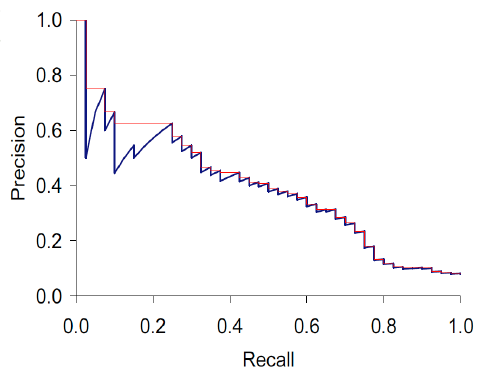
\includegraphics[width = \textwidth]{./images/preciseFunction.png}	
					\end{minipage}
					\begin{minipage}{0.45\textwidth}
						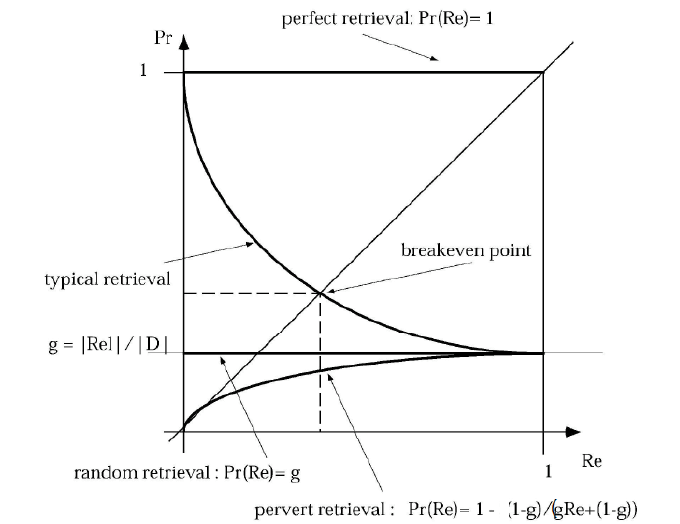
\includegraphics[width = \textwidth]{./images/asymptFunction.png}
					\end{minipage}
				\end{figure}

		\subsection{Information Retrieval Process}
			Documents in a collection must be abstracted in some logic way. The most naive way to provide a \underline{logical view} of a document is to see it as a set of index terms and keywords through \textbf{text operations}. Then, the keywords are used to index the documents and the generated indexes are used to speed up searching operations. We can so identify and \textit{indexing process} that is divided in a keyword search (inside the document) adn then the building of an index upon such keywords.
			
			\subsubsection{Text Processing}
				Processing a text document is composed of several task:
				\begin{enumerate}
					\item parsing: turning a document with a characters stream. This deals with format issues, language issues, characters sets issues...
					\item lexical analysis: this part of the process transforms the input characters streams into a set of recognized words (the \textbf{tokens}). These are \textit{candidated keywords}; the lexical analysis deals with tokenization issues such as recognizing the separators, the lexical units, how to manage cases, punctuation...
					\item elimination of stopwords: a stopword is a word that occurs multiple times in a document. These are intend as the useless additional conjunction, adverbs, articles etc. This is a super delicate process: we can decrease significantly recall (web searches do not remove stopwords)
					\item phrases identification: this step "groups nouns" together to identify phrases. This operation is done with the help of a thesaurus (or multiple ones) that brings a vocabulary alongside a set of phrases and phrases patterns to match to.
					\item stemming and lemmanizations: "reduce the terms to their roots". This procedure associates the words to their base form by reducing the inflections and variations. Some stemmers also chops the words directly to their roots (producing so a "meaningless" text where all the words have not suffixes of prefixes, even the plural ones). This is done in order to reduce the document to just a list of keywords.
						\begin{itemize}
							\item \textbf{stemming} is the procedure to chopping the words in an attempt to find the root
							\item \textbf{lemmanization} instead tries to return (again with thesauruses and known tables) words and tokens to their "semantic" root, as returning a past tense to a base form
						\end{itemize}
					\item term weighting: after having identified all the relevant words and tokens and index-usable words, we can also \textit{weight} them on an "importance" scale, in order to provide even further information with the document.
						\begin{itemize}
							\item Zipf's law: an empirical law that states \textit{the frequency of a word is inversely proportional to its rank}. We can so define a function, for each word \emph{w} that links its frequency and its rank: $r(w)\, \times\, f(w)\, =\, c$, where \emph{c} is an arbitrary constant (usually language-dependent)
							\item Luhn's analysis is another empirical law that maximizes the weight of a word accounting also the position in the phrase other than his frequency of appearance
						\end{itemize}
				\end{enumerate}

			\subsubsection{Data Structures}
				Basically, we need data structures to hold our seearch result and intermediate values. A first simple approach is to link documents and tokens with a matrix: it would be a super sparse matrix, lot of wasted terms.\\
				Another approach is the "inverted index": we hold a dictionary of tokens and \textit{for each token} we memorize the document (and the positions in such documents) where the token appears. The opportunity to dinamically allocate slots in an inverted index and the speed of retrieving information inside them makes them the \textit{best data structure} to support text information retrieving.\\
				Trees can also be used (as they're used as search structures in DBs) to speed up information retrieval. The most used kind is the highest performing B+ tree format.

			\subsubsection{IR Strategies}
				A retrieval strategy is an algorithm that takes a query and have to return documents that match \textit{at a certain level} the specified query.

				\paragraph{Boolean Model}
					We use boolean algebra to build our query. It's very simple: we combine logically the keywords (with classic boolean operators as AND, NOT) and we find the documents that match the query, now expressed as a boolean formula. Boolean queries are usually expressed (or tansformed) in disjunctive normal form; from the inverted indexes are retireved the posting lists of documents that then are analyzed to find a match. The big cons of the boolean model is that it does not support any kind of ranking.

				\paragraph{Vector Model}
					The vector model represents documents and queries as vectors in the term space. Terms weights are used to compute the \textit{similarity} of the query and the document and assign a score. The "term space" is a n-dimensional space where each axis is a token: each document is "located" in such space accounting for the number of times a token appears in it (this can be used as a weight measure) and representing it as a vector. To match a query to a document we should use a non-euclidean notion of distance, for example the so called "cosine similarity" measure.\\
					The weighting mechanism is very delicate: we should normalize regarding to the document's lenght, the document's type, the total number of different tokens etc... The go-to index for weighting a toke is $w_{id} = tf_{id} \times idf_{i}$ where
					\begin{itemize}
						\item $tf_{i, d}$ is the frequency with which term \emph{i} appears in document \emph{d}
						\item $idf_i$ inverse document frequency of term \emph{i}: this term is high for rare terms, and keeps into account the \textit{number of documents in which they appear}
					\end{itemize}
					so, in the end, $w_{i, d}$ grows with the number of occurrences within a doc and with the rarity of the term among the whole collection.\\
					The main drawback of this model is the difficult way in which a structured query must be generated: no AND, OR, NOT operators are provided. Also, it's far more demanding in computational power due to the complex vector representation.

				\paragraph{Probabilistic Model}
					With this approach we want to compute the probability that a given document will be relevant to a query. This model is \textit{interactive}, as it requires the user to interact for some time refining the results (and our idea of probability). Most of the times we would not have a user, so we go through
					\begin{enumerate}
						\item we assume all the probabilities are the same (uniform distribution)
						\item we sort the documents with a weight (number of appearance of a token...)
						\item we extract the "relevant ones" setting a number of useful documents from the first in the list
						\item update the statistics after this last step
						\item return to step 2 until convergence						
					\end{enumerate}
		
		\subsection{Document Clustering}
			Clustering is another approach to IR that organizes documents in "clusters" that represents the "family" of documents, grouping them for similarity. This problem boils down to fix a number of clusters and an objective function that evaluates the quality of the clustering, and then maximize the objective function. Usually this function aims to not leave any cluster empty. Again, we evaluate the similarity of two documents with indixes as \textbf{topic similarity} or \textbf{common high values} for certain tokens.
					
	\section{Web Information Retrieval}
		\subsection{Search Engines}
			Search engines are associative search infrastructures whose purpose is to retrieve information using keywords.\\
			A search engine needs a model of the Web, in order to practically and easily crawl through it. The classical representation is a Graph, and specifically a \textit{scale free} network, that is characterized by a \textit{power distribution} for the number of edges for each node: there's a very high probability that a node has "a few" links, and a low probability that a node has "a lot" of links. In such a graph we can identify Thematically Unified Clusters. The web can be also seen as a fractal-bowtie structure, so a series of strongly connected components that link all the content, but this is true for many scales: the micro and the macro organization of the web behaves the same.\\
			This structure helps characterize node, by properties as \textit{centrality, prestige, rank} etc...

		\subsection{Web Crawling}
			For "web crawler" or "web spider" is intended a software component that goes through documents (in this case, it's specialized in web pages) in order to build indexes and \textit{quickly provide results}.\\
			A crawler must be
			\begin{itemize}
				\item \textbf{robust}, it should avoid endless looping
				\item \textbf{polite}, it should respect web server policies
				\item distributed
				\item scalable
				\item quality and freshness centric for results				
			\end{itemize}
			Crawlers works in a very easy way: HTTP requests to a web site then analyzes the content, that's 99\% of the time described in some markup language (HTML, XML...). The crawler \textit{embeds} a module that carries out each step of the text analysis procedure, it contains a parser, a tokenizer etc; all this modules exist alongside the web-related modules, such a policy interpreter for web servers.

			\paragraph{Robot Exclusion Protocol}
				It has became more and more in use a REP that a website owner can abilitate on his site in order to facilitate the crawler's job on it: it signals the portions that the crawler should skip in order to efficently index that site. It is an \textit{advisory} measure, a crawler could ignore it.

			\paragraph{Sitemaps}
				Crawlers can use \textit{formatted sitemaps} in order to efficently navigate a site. This other protocol was proposed by Google itself. The sitemap can be formatted in every formal language or representation and (alongside REP) speeds up the crawling procedure.

			\subsubsection{Crawler Architecture}
				A crawler is composed by several interconnected modules, each one carrying out a specific task:
				\begin{figure}[H]
					\centering
					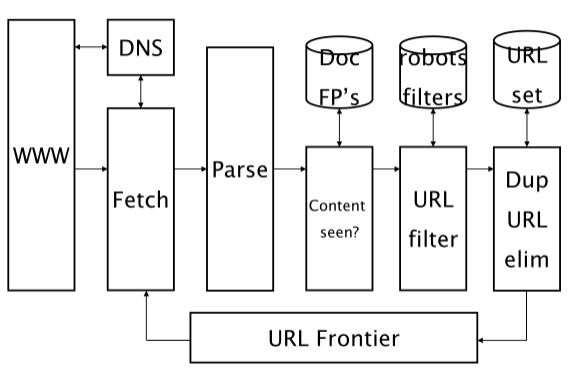
\includegraphics[width = \textwidth]{images/crawlerArchitecture.png}
				\end{figure}
				the names of the modules are pretty straightforward, but in detail:
				\begin{itemize}
					\item the DNS resolver queries the DNS service, it's the "navigation" module of the crawler
					\item the \underline{url frontier} is the set of URLs yet to be fetched in this run
					\item fetcher and parser respectively retrieve the page and extract the relevant information
					\item URL filters extracts the "useful" URLs from the page (also checking the site policies)
				\end{itemize}
				To distribute such an architecture, we need to insert a module "host splitter" between the URL filter and the Duplicate elimination, in order to synchronize all the crawler processes.

			\subsubsection{Spider Traps and Crawler Fairness}
				Spider traps are (quite straightforwardly) URL loops that can "trap" a crawler in an endless circle. This happens, for example, when a page dynamically creates and handles the URLs it's redirecting to. An option is to randomly "jump away" from a URL, or to reduce the lenght of the maximum URL that can be processed.\\
				Crawler fairness: some crawler can put in place behaviours (like randomizing the input to pages to mimic the user, or slow the requests rate, or use a false user agent etc). Fairness is also intended in the other way: a site can put in place cloaking techniques to avoid being crawled. 

		\subsection{Link Analysis}
			Link analysis is the idea to use also hyperlinks (alongside content) to rank the pages in the web. The \textit{anchor text} plays a special role in link analysis: how another page is described? The description of the link is useful to extract information about the target page.

		\subsection{PageRank}
			Page ranking is the procedure to assign a score (a numerical value) to a document basing on some other data or properties, as
			\begin{itemize}
				\item ingoing links
				\item outgoing links (not optimal: gaining score "doing nothing")
				\item both: each "vote" from a page to another is weighted against the number of total outgoing links from it. Computing the score then boils down to solving a linear system in the classic $A \cdot x = x$ form. \emph{A} represents the \underline{weighted adjacency matrix} of the web portion we're considering. The converged score is found at convergence point at $\lim_{k \rightarrow \infty} A^k$
			\end{itemize}
			In a way, this is a democratic scoring mechanism, because each page is \textit{objectively evaluated}.

			\subsubsection{Random Surfer Interpretation}
				In not strongly connected graphs (very sparse adjacency matrixes) the value of the score, so the \emph{x} vector, could be \underline{not unique}, as the result of a linear system with a lot of zeroes\footnote{obiously corresponding to the missing links between pages}. To avoid multiple "conflicting" score configurations and to interpret the matrix \emph{A} as a \underline{probability of visit} matrix (imagine a random-based crawler that follows the probability matrix to jump) we can generate another matrix as $M = (1-m) \cdot A + m \cdot S$ where \emph{m} is called \textit{damping factor} and represents "fake links" among all pages, while \emph{S} is a homogeneous matrix where each entry is just $\frac{1}{number\,of\, pages}$

			\subsubsection{Markov Chain Interpretation} %%TODO

			\subsubsection{Timed Page Rank}
				Outdated pages are obviously less interesting (not up to date), but they will still be ranked in the matrix. This can be taken into account by adding the time into the equation calulating the \textit{weight of the vote}, using a damping factor that increases with time.

		\subsection{HITS}
			Hypertext Induced Topic Search is a search system that depends on text-based queries that has a peculiar internal architecture for the link analysis: each page can either be
			\begin{enumerate}
				\item a hub, that links to good authorities
				\item an authority, that links to good hubs
			\end{enumerate}
			each page has a double rank, a hub score and an authority score, computed by the number of (respectively) outgoing and ingoing links. The algorithm is similar to the previous ones, computing a matrix by power iterating over it. The idea behind the search then becomes "good hubs points to good authorities, good authorities are pointed by good hubs".
		
			\subsubsection{HITS vs PageRank} %%TODO

	\section{Google's Interaction Experience}
		%%TODO

\end{document}



































